\documentclass[a4paper,10pt,landscape]{article}

% document setup
\usepackage[left=7mm,right=7mm,top=15mm,bottom=7mm,landscape]{geometry} % margin = .. total={280mm,190 mm} % in geometry for defined size/ratio
\usepackage{multicol,multirow}
\usepackage[utf8]{inputenc} % not strictly necessary, but sets utf8

% enable colors
\usepackage{xcolor,color} % standard colors (blue, red, etc.https://www.namsu.de/Extra/pakete/Xcolor.html )

% multicol settings
\setlength{\premulticols}{1pt}
\setlength{\postmulticols}{1pt}
\setlength{\multicolsep}{1pt}
\setlength{\columnsep}{5pt}
\setlength{\columnseprule}{1pt}
\def\columnseprulecolor{\color{black}}

% language
\usepackage[english]{babel} %choose your language

% for images
\usepackage{graphicx}
\graphicspath{ {./images/} }

% Images combined with texts
\usepackage{wrapfig}

% some AsmTeX options
\usepackage{amscd, amsmath,amssymb}

% more fine control for lists
\usepackage{enumitem}

% multiple line comments and testing text
\usepackage{comment} % \begin{comment} \end{comment} 
\usepackage{blindtext} % inserts lorem ipsum like text

% table that supports equations
\usepackage{tabularx}

% hyperlinks (has to be after titlesec, else we get errors
\usepackage[colorlinks=true,citecolor=blue,linkcolor=blue,urlcolor=black]{hyperref}

% Example section environment
\newenvironment{examplesection}[1][]
    {
        \subsubsection{#1}
        \color{blue}
    }
    {
    }

% define header style
\usepackage[headsepline]{scrlayer-scrpage}
\pagestyle{scrheadings}
\ihead{Signal- und Systemtheorie I - \today}
\chead{\pagemark}
\ohead{\url{https://github.com/MeierTobias/eth-sigsys-1}}
% colors
\usepackage{color,xcolor}
\definecolor{sectionColor}{HTML}{1c59c9}
\definecolor{subSectionColor}{HTML}{568ae8}
\definecolor{subSubsectionColor}{HTML}{87a9e8}
\definecolor{titleTextColor}{RGB}{255,255,255}

% set the size of a section
\usepackage{parskip}
\setlength{\parindent}{0pt}
\setlength{\parskip}{0pt}

% used for colored boxes
\usepackage[many]{tcolorbox}

% customize the headers
\usepackage[explicit]{titlesec}

\titleformat{\section}
{\normalfont\bfseries\fontfamily{lmss}\selectfont}
{}
{0pt}
{\begin{tcolorbox}[
      enhanced,
      boxrule=0pt,
      arc=0pt,
      outer arc=0pt,
      left=0pt,
      right=0pt,
      top=0pt,
      bottom=0pt,
      nobeforeafter,
      interior code={\fill[overlay,sectionColor] (frame.north west) rectangle (frame.south east);},
    ]\textcolor{titleTextColor}{\thesection\hspace{0.5em}#1}
  \end{tcolorbox}}
\titlespacing{\section}{0pt}{0pt}{0pt}

\titleformat{\subsection}
{\normalfont\bfseries\fontfamily{lmss}\selectfont}
{}
{0pt}
{\begin{tcolorbox}[
      enhanced,
      boxrule=0pt,
      arc=0pt,
      outer arc=0pt,
      left=0pt,
      right=0pt,
      top=0pt,
      bottom=0pt,
      nobeforeafter,
      interior code={\fill[overlay,subSectionColor] (frame.north west) rectangle (frame.south east);},
    ]\textcolor{titleTextColor}{\thesubsection\hspace{0.5em}#1}
  \end{tcolorbox}}
\titlespacing{\subsection}{0pt}{0pt}{0pt}

\titleformat{\subsubsection}
{\normalfont\bfseries\fontfamily{lmss}\selectfont}
{}
{0pt}
{\begin{tcolorbox}[
      enhanced,
      boxrule=0pt,
      arc=0pt,
      outer arc=0pt,
      left=0pt,
      right=0pt,
      top=0pt,
      bottom=0pt,
      nobeforeafter,
      interior code={\fill[overlay,subSectionColor] (frame.north west) rectangle (frame.south east);},
    ]\textcolor{titleTextColor}{\thesubsubsection\hspace{0.5em}#1}
  \end{tcolorbox}}
\titlespacing{\subsubsection}{0pt}{0pt}{0pt}

%-----------------------------------------------------%
% for colours
\usepackage{color}
% from code expert "ce_"
\definecolor{ce_yellow}{rgb}{0.902,0.859,0.455}
\definecolor{ce_gray}{rgb}{0.459,0.443,0.369}
\definecolor{ce_lime}{rgb}{0.459,0.816,0.180}
\definecolor{ce_pink}{rgb}{0.976,0.149,0.447}
\definecolor{ce_cyan}{rgb}{0.40,0.851,0.937}
\definecolor{ce_violet}{rgb}{0.545,0.506,1.00}
\definecolor{ce_back}{rgb}{0.153,0.157,0.133}
\definecolor{ce_white}{rgb}{1,1,1}
%----------------------------------------------------%
% as close to CodeExpert as i could get it
\usepackage{listings}

\lstdefinestyle{CodeExpert}{
    language=C++,
    basicstyle=\ttfamily\linespread{0.8}\color{ce_white},
    numbers=none,
    aboveskip=0mm,
    belowskip=0mm,
    frame = none,
    numberstyle=\tiny\color{ce_grey},
    backgroundcolor = \color{ce_back},
    keywordstyle=\color{ce_cyan},
    commentstyle=\color{ce_gray},
    stringstyle=\color{ce_yellow},
    morecomment=[n][\color{ce_pink}]{\#}{\ },
    literate=
    *{./}{{{\color{ce_pink}./}}}2
    {.^}{{{\color{ce_pink}.\^{}}}}2
    {=}{{{\color{ce_pink}=}}}1
    {+}{{{\color{ce_pink}+}}}1
    {*}{{{\color{ce_pink}*}}}1
    {-}{{{\color{ce_pink}-}}}1
    {&}{{{\color{ce_pink}&}}}1
    {<<}{{{\color{ce_pink}<<}}}2
    {>>}{{{\color{ce_pink}>>}}}2
    {<}{{{\color{ce_pink}<}}}1
    {>}{{{\color{ce_pink}>}}}1
    {->}{{{\color{ce_pink}->}}}2
    {1}{{{\color{ce_violet}1}}}1
    {2}{{{\color{ce_violet}2}}}1
    {3}{{{\color{ce_violet}3}}}1
    {4}{{{\color{ce_violet}4}}}1
    {5}{{{\color{ce_violet}5}}}1
    {6}{{{\color{ce_violet}6}}}1
    {7}{{{\color{ce_violet}7}}}1
    {8}{{{\color{ce_violet}8}}}1
    {9}{{{\color{ce_violet}9}}}1
    {0}{{{\color{ce_violet}0}}}1
    {this}{{{\color{ce_lime}this}}}1
    {if}{{{\color{ce_pink}if}}}1
    {do}{{{\color{ce_pink}do}}}1
    {for}{{{\color{ce_pink}for}}}1
    {else}{{{\color{ce_pink}else}}}1
    {then}{{{\color{ce_pink}then}}}1
    {break}{{{\color{ce_pink}break}}}1
    {continue}{{{\color{ce_pink}continue}}}1
    {public}{{{\color{ce_pink}public}}}1
    {private}{{{\color{ce_pink}private}}}1
    {while}{{{\color{ce_pink}while}}}1
    {continue}{{{\color{ce_pink}continue}}}1
    {nullptr}{{{\color{ce_violet}nullptr}}}1
    {NULL}{{{\color{ce_violet}NULL}}}1,
}

\lstset%
    {
    basicstyle=\ttfamily,
    frame=tb,
    aboveskip=1mm,
    belowskip=1mm,
    showstringspaces=true,
    columns=flexible,
    breaklines=true,
    breakatwhitespace=true,
    tabsize=2,
}
%Mathematik-Pakete
\usepackage{amsmath, amstext, amssymb, mathtools, esint, polynom, trfsigns, pgfplots}
\usepackage{bm}
\allowdisplaybreaks %Seitenumbruch in align-Umgebung erlauben
%

%Definition der Umgebung "example"
\newenvironment {example}
				{\begin{itshape} \begin{small}}
				{\end{small} \end{itshape}}
%				
%Definition der Umgebung "annotation"		
\newenvironment {annotation}[1]
				{\begin{itshape} \begin{small} \textbf{#1} \begin{itemize}}
				{\end{itemize} \end{small} \end{itshape}}
%				
%Definition der Umgebung "eq"
\newenvironment {eq}
				{\begin{equation*}}
				{\end{equation*}}
%
% Don't know what this does
\providecommand{\diff}{\mathop{} \! \mathrm{d}}
\DeclareMathOperator{\rot}{rot}
\DeclareMathOperator{\divg}{div}
%\excludecomment{examplesection}

\begin{document}
\begin{multicols*}{3}

    \begin{center}
        \huge{Signal- und Systemtheorie I \par}
        \vspace{0.1cm}
        \large{HS23 ETHZ\par}
        \vspace{0.3cm}
        \normalsize{Tobias Meier}
        \vspace{0.3cm}
    \end{center}
    {
    Der Grossteil dieser Zusammenfassung basiert auf Auszügen des Vorlesungsskriptums von Herrn Prof.\ Dr.\ Bölcskei.\newline{}
    Dieses PDF, der Quellcode sowie der Disclaimer können dem nachfolgenden GitHub Repository entnommen werden: \url{https://github.com/MeierTobias/eth-sigsys-1}
    }
    \vspace{0.2cm}

    \section{Anwendungen der Signal und Systemtheorie}
% keine Zusammenfassung


    \section{Einteilung der Signale}
% keine Zusammenfassung


    \section{Lineare Räume}


    \section{Systeme und Systemeigenschaften}


    \section{Analoge lineare zeitinvariante Systeme im Zeitbereich}


    \section{Verallgemeinerte Funktionen}


    \section{Analoge lineare Systeme im Frequenzbereich}
\subsection{Eigenfunktionen}

\begin{center}
    \begin{tikzpicture}[auto, node distance=2cm,>=latex']
        \node [input, name=rinput] (rinput) {};
        \node [block, right of=rinput] (h1) {$H$};
        \node [output, right of=h1, node distance=2cm] (output) {};
        \draw [->] (rinput) -- node{$x(t)$} (h1);
        \draw [->] (h1) -- node [name=y] {$y(t)$}(output);
    \end{tikzpicture}
\end{center}

Die Funktionen $e^{2\pi{}ift}$ sind Eigenfunktionen des Systems H, die zugehörigen Eigenwerte sind $\hat{h}(f)$. Der Frequenzgang des LTI-Systems ist gleich der Fouriertransformation $\hat{h}(f)$ der Impulsantwort $h(t)$.

\begin{align*}
    Hx               & =\lambda{}x                  \\
    He^{2\pi{}if_0t} & =\hat{h}(f_0)e^{2\pi{}if_0t}
\end{align*}

\textbf{Analogie zu Eigenvektoren und Eigenwerten von Matrizen.}
Es sei $H \in \mathbb{C}^{n\times{}n}$ eine Matrix mit der nachfolgenden Eigenwertzerlegung.
\begin{equation*}
    H=U\Sigma{}V^H
\end{equation*}
Wenn H normal ist ($HH^H=H^HH$):
\begin{equation*}
    H=U\Sigma{}U^H=\sum_{i=1}^{n}u_i\lambda_iu_i^H=\color{section}{\sum_{i=1}^{n}\lambda_iu_iu_i^H}\\
\end{equation*}
Dabei ist
\begin{equation*}
    UU^H = U^HU=I_n \Leftrightarrow \langle{}u_i,u_j\rangle{}=
    \begin{cases}
        1, & i=j           \\
        0, & \text{sonst.}
    \end{cases}
\end{equation*}
Wird die Matrix mit einem Eigenvektor "angeregt", so erhalten wir
\begin{align*}
    Hu_\ell & ={\color{section}{\left(\sum_{i=1}^n\lambda_iu_iu_i^H\right)}}u_\ell=\sum_{i=1}^n\lambda_iu_i\underbrace{(u_i^Hu_\ell)}_{=\delta_{i-\ell}} \\
    Hu_\ell & =\lambda_\ell{}u_\ell
\end{align*}

Wenn wir den Vektor $x$ als Linearkombination der Basisvektoren $u_i$ schreiben
\begin{equation*}
    x=\sum_{i=1}^{n}c_iu_i, \text{mit Koeffizienten} c_i=\langle{}x,u_i\rangle
\end{equation*}
Dann erhält man für das Ausgangssignal
\begin{align*}
    Hx & ={\color{section}{\left(\sum_{i=1}^n\lambda_iu_iu_i^H\right)}} \sum_{j=1}^nc_ju_j \\
       & =\sum_{i=1}^n\sum_{j=1}^n\lambda_ic_ju_i\underbrace{u_i^Hu_j}_{=\delta_{i-j}}     \\
       & =\sum_{i=1}^n\lambda_ic_iu_i
\end{align*}
Diese Darstellung entspricht der zuvor abgeleiteten Beziehung für zeitkontinuierliche Systeme
\begin{equation*}
    (Hx)(t)=\int_{-\infty}^\infty\underbrace{\hat{h}(f)}_{\lambda_i}\underbrace{\hat{x}(f)}_{c_i=\langle{}x,u_i\rangle}\underbrace{e^{2\pi ift}}_{u_i}df
\end{equation*}

\subsubsection{Kaskadierung}
\begin{center}
    \begin{tikzpicture}[auto, node distance=2cm,>=latex']
        \node [input, name=rinput] (rinput) {};
        \node [block, right of=rinput] (h1) {$H_1$};
        \node [block, right of=h1] (h2) {$H_2$};
        \node [output, right of=h2, node distance=2cm] (output) {};
        \draw [->] (rinput) -- node{$x(t)$} (h1);
        \draw [->] (h1) -- node{$y_1(t)$} (h2);
        \draw [->] (h2) -- node [name=y] {$y(t)$}(output);
    \end{tikzpicture}
\end{center}
\begin{align*}
    h(t)    & =(h_1*h_2)(t)       \\
    \hat{h} & =\hat{h_1}\hat{h_2}
\end{align*}

\subsubsection{Weitere spezielle Eingangssignale}
\textbf{Allgemeine Schwingungen:}
\begin{align*}
    x(t)   & =e^{st}             \\
    \intertext{mit}
    s      & =\sigma + i2\pi f_0 \\
    \Re(s) & = \sigma
    \begin{cases}
        <0, & \text{zeitlich abklingende Einhüllende} \\
        =0, & \text{zeitlich konstante Einhüllende}   \\
        >0, & \text{zeitlich anklingende Einhüllende}
    \end{cases}
\end{align*}
Das zugehörige Ausgangssignal lässt sich in diesem Fall schreiben als
\begin{equation*}
    y(t)=(x*h)(t)=\int_{-\infty}^\infty h(\tau)e^{s(t-\tau)}d\tau=e^{st}\underbrace{\int_{-\infty}^\infty h(\tau)e^{-s\tau}d\tau}_{=:H(s)}
\end{equation*}
wobei $H(s)$ die Laplacetransformierte von $h(t)$ genannt wird.

\bigskip

\textbf{Sinusförmiges Eingangssignal}
\begin{equation*}
    x(t)=\cos(2\pi f_0t+\varphi_0)=\frac{1}{2}e^{2\pi if_0t}e^{i\varphi_0}+\frac{1}{2}e^{-2\pi if_0t}e^{-i\varphi_0}
\end{equation*}
Ausgangssignal:
\begin{equation*}
    y(t)=\frac12\hat{h}(f_0)e^{2\pi if_0t}e^{i\varphi_0}+\frac12\hat{h}(-f_0)e^{-2\pi if_0t}e^{-i\varphi_0}
\end{equation*}
Für $h(t)\in\mathbb{R}$ gilt $\hat{h}(f)=\hat{h}^*(-f)$ und somit
\begin{equation*}
    y(t) = |\hat{h}(f_0)|\cos(2\pi f_0t+\varphi_0+\arg\hat{h}(f_0))
\end{equation*}
$|\hat{h}(f)|$ gibt die Änderung der Amplitude und $arg(\hat{h}(f))$ die Änderung der Phase gegenüber
dem Eingangssignal an.

\subsection{Die Fouriertransformation}
Definition:
\begin{equation*}
    \hat{x}(f):=(\mathcal{F}x)(f):=\int_{-\infty}^\infty x(t)e^{-2\pi ift}dt
\end{equation*}
Rücktransformation
\begin{equation*}
    x(t):=(\mathcal{F}^{-1}\hat{x})(t):=\int_{-\infty}^\infty\hat{x}(f)e^{2\pi ift}df
\end{equation*}

\smallskip

\textbf{Riemann-Lebesgue Lemma}

Es sei $x$ ein absolut integrierbares Signal, d.h. $x \in L^1$. Dann ist $(\mathcal{F}x)(f)=\hat{x}(f)$ stetig und es gilt $\lim_{|f|\to\infty}(\mathcal{F}x)(f)=0$.

\subsubsection{Fouriertransformation verallgemeinerter Funktionen}
oder Funktionen die weder in $L^1$ noch in $L^2$ sind (z.B. $x(t)=1$ oder $x(t)=e^{i2\pi at}$).
\\
\textbf{Plancherelsche Identität}
Es sei $x,y \in L^2$
\begin{align*}
    \int_{-\infty}^\infty x(t)y^*(t)dt & =\int_{-\infty}^\infty\hat{x}(f)\hat{y}^*(f)df \\
    \langle x,y\rangle                 & = \langle\hat{x},\hat{y}\rangle
\end{align*}
Diese Gleichung dient als Grundlage zur Erweiterung des bisherigen Testfunktionenraums $\mathcal{D}$ auf den linearen Raum $\mathcal{S}$ aller beliebig oft differenzierbaren Funktionen, die gemeinsam mit jeder Ableitung für $|u| \rightarrow \infty$ stärker als jede Potenz von $1/|u|$ gegen Null gehen. Der resultierende Testfunktionenraum, genannt $\mathcal{S}$, enthält alle bisher betrachteten Testfunktionen und hat die Eigenschaft, dass für jede Funktion $\varphi \in \mathcal{S}$ auch $\hat{\varphi} = \mathcal{F}\varphi \in \mathcal{S}$. Ein Funktional auf $\mathcal{S}$ wird als temperierte verallgemeinerte Funktion bezeichnet.
Somit kann gezeigt werden, dass gilt:
\begin{align*}
    \ell_x(\hat{\varphi})      & =\ell_{\hat{x}}(\varphi)   \\
    \ell_x(\mathcal{F}\varphi) & =\ell_{\mathcal{F}x}(\ell) \\
    \ell(\mathcal{F}\varphi)   & =:\mathcal{F}\ell(\varphi)
\end{align*}
\begin{equation*}
    \mathcal{F}\ell_x(\varphi):=\ell_x(\mathcal{F}\varphi)=\ell_{\mathcal{F}x}(\varphi)
\end{equation*}
Folgende Eigenschaften gelten auch für $\varphi \in \mathcal{S}$:
\begin{align*}
     & \text{Additivität}     &  & (\ell+\widetilde{\ell})(\varphi):=\ell(\varphi)+\widetilde{\ell}(\varphi) \\
     & \text{Homogenität}     &  & (\alpha\ell)(\varphi):=\alpha\ell(\varphi)                                \\
     & \text{Zusammensetzung} &  & (\ell\circ g)(\varphi):=\frac{1}{|a|}\ell(\psi),                          \\
     &                        &  & \psi(t)=\varphi\!\left(\frac{t-b}{a}\right),\quad g(t)=at+b               \\
     & \text{Multiplikation}  &  & (\psi\ell)(\varphi):=\ell(\psi\varphi)
\end{align*}
wobei für die Multiplikation noch die Einschränkung hinzukommt, dass $\phi(t)$ für $|t| \rightarrow \infty$ nicht allzu stark wachsen darf, damit auch $\psi(t)\varphi(t) \in \mathcal{S} $.
Des weiteren bleibt für die Differentiation gültig:
\begin{align*}
     & \text{Ableitung}    &  & D\ell(\varphi)=\ell'(\varphi):=-\ell(\varphi')                           \\
     & \text{Additivität}  &  & (\ell+\tilde{\ell})'(\varphi):=\ell'(\varphi)+\widetilde{\ell}'(\varphi) \\
     & \text{Homogenität}  &  & (\alpha\ell)'(\varphi):=\alpha\ell'(\varphi)                             \\
     & \text{Produktregel} &  & (\psi\ell)'=\psi'\ell+\psi\ell'
\end{align*}

\textbf{Vorgehen:}

Auf verallgemeinerte Funktionen $\ell$ anwenden damit auch nicht absolut integrierbare Funktionen verwendet werden können.
\begin{align*}
    y               & =\mathcal{F}x                                            \\
                    & \downarrow \ell                                          \\
    \ell_y(\varphi) & =\ell_{\mathcal{F}x}(\varphi)=\ell_x(\mathcal{F}\varphi)
\end{align*}

\textbf{Einige Fouriertransformationspaare:}
\begin{align*}
    \delta(t) \;                                 & \laplace\; 1                                                        \\
    sign(t) \;                                   & \laplace\; \frac{1}{\pi if}                                         \\
    \Sigma(t) \;                                 & \laplace\; \frac{1}{2\pi if}+\frac{1}{2}\delta(f)                   \\
    e^{2\pi iat} \;                              & \laplace\; \delta(f-a)                                              \\
    sin(2\pi f_0t) \;                            & \laplace\; \frac{i}{2}\left(\delta(f+f_0)-\delta(f-f_0)\right)      \\
    cos(2\pi f_0t) \;                            & \laplace\; \frac{1}{2}\left(\delta(f+f_0)+\delta(f-f_0)\right)      \\
    \sum_{k=-\infty}^\infty c_ke^{2\pi ikt/T} \; & \laplace\; \sum_{k=-\infty}^\infty c_k\delta\left(f-\frac kT\right)
\end{align*}
Es folgen weitere Beziehungen, die für verallgemeinerte Funktionen ihre Gültigkeit bewahren:
\begin{align*}
    (\mathcal{F}^2x)(f)                             & = x(-f)                                                                     \\
    \left((\mathcal{F}^{-1})^2\widehat{x}\right)(t) & = \hat(-t)                                                                  \\
    x(t-t_{0}) \;                                   & \laplace\; e^{-2\pi ift_0}\hat{x}(f)                                        \\
    x(at+b) \;                                      & \laplace\; \frac{1}{|a|}\int_{-\infty}^{\infty}x(t')e^{-2\pi if(t'-b)/a}dt' \\
                                                    & =\frac1{|a|}e^{i2\pi fb/a}\hat{x}(f/a)                                      \\
    e^{2\pi if_{0}t}x(t) \;                         & \laplace\; \hat{x}(f-f_0)
\end{align*}

\textbf{Die Fouriertransformation als Rotation in der Zeit-Frequenz-Ebene:}
\begin{center}
    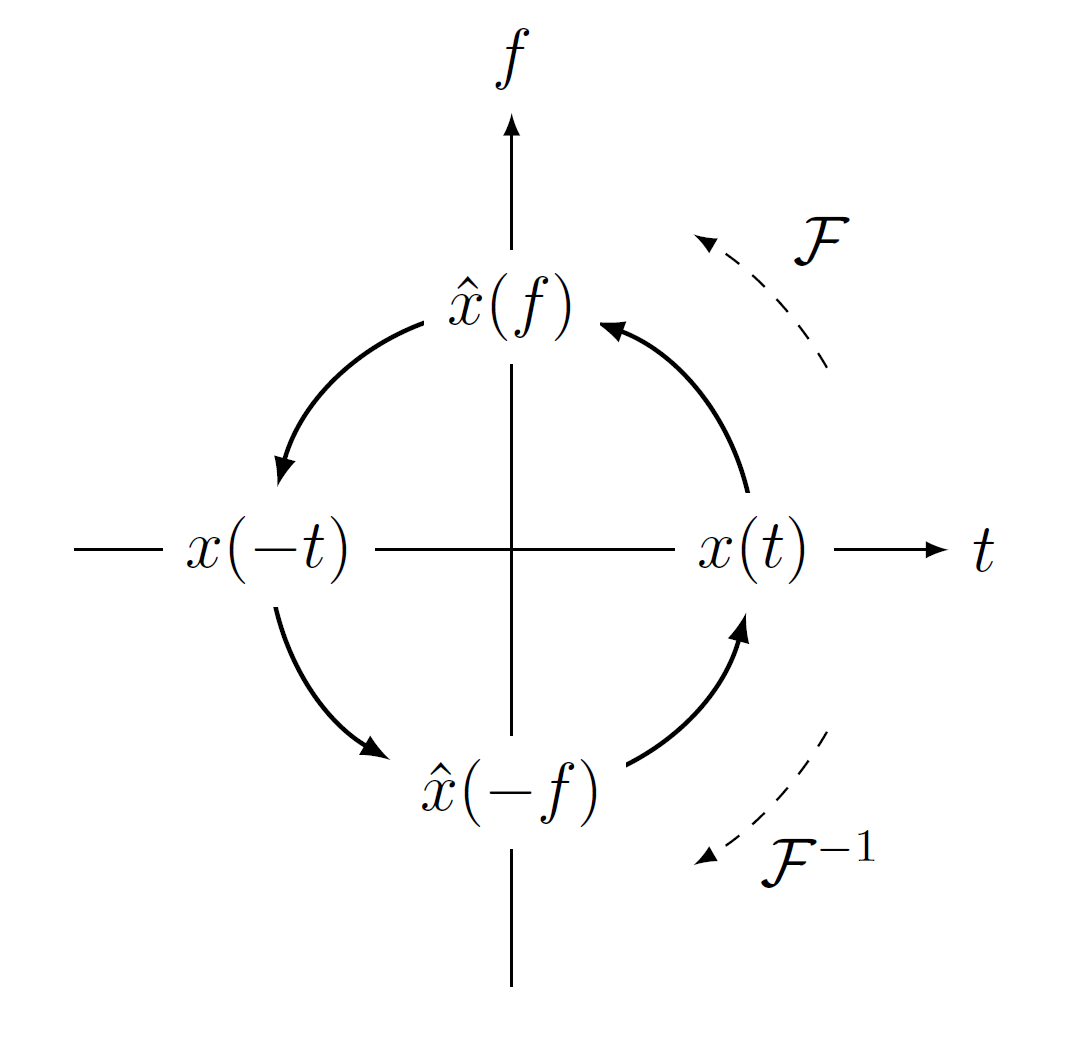
\includegraphics[width=0.6\linewidth]{img/FT_Rotation.png}
\end{center}
\begin{align*}
    x(t) \;       & \laplace\; \hat{x}(f)  \\
    \hat{x}(t) \; & \laplace\; x(-f)       \\
    x(-t) \;      & \laplace\; \hat{x}(-f) \\
    \hat{x}(-t)\; & \laplace\; x(f)
\end{align*}

\textbf{Differentiation}
\begin{equation}
    \mathcal{F}x'=2\pi if\mathcal{F}x=2\pi if\hat{x}
\end{equation}

\textbf{Faltung verallgemeinerter Funktionen}
\begin{equation}
    (\mathcal{F}(x*y))(f) = \hat{x}(f)\hat{y}(f)
\end{equation}

    \section{Abtasttheorem}


    \section{Zeitdiskrete Signale und Systeme}


    \section{Die diskrete Fouriertransformation DFT}


    \section{Die schnelle Fouriertransformation FFT}


    \section{Anhang}


    % a model columnbreak
    % \vfill\null % prevents the columns content from using the full height
    % \columnbreak
    %

\end{multicols*}

\end{document}